% !TeX root = ../artigo.tex
\section{MATERIAL E MÉTODOS}

O desenvolvimento do projeto proposto, demandou a instalação e configuração de uma máquina virtual Debian, dentro de um servidor Proxmox. Para isso, foram seguidas as etapas recomendadas para garantir uma implementação adequada e funcional.

Para a instalação do Proxmox, foi realizado o uso de hardware compatível com seus requisitos mínimos \cite{proxmox-requirements}. O hardware usado para sua implementação foi: um processador Intel Xeon E-2336 @ 2.90GHz, memória RAM de 16 GB e um disco rígido com 64 GB de espaço.

Após verificada a estabilidade da versão escolhida do Proxmox, foi realizado o procedimento de instalação padrão do Proxmox VE 7.4, que incluiu o download da imagem ISO, criação de uma mídia de instalação (DVD ou USB), inicialização do servidor a partir da mídia e execução do assistente de instalação. Foram fornecidas as informações necessárias, como configurações de rede adequadas, senhas de acesso e seleção do disco para uma instalação eficiente.

Com a instalação do servidor Proxmox bem sucedida, foi prosseguida a implementação da máquina virtual, que contém a versão 12.1.0 do Debian, instalada como CLI, possuindo 2GB de memória RAM e 32GB de armazenamento, como ilustrado na Figura \ref{fig:hardwareDebian} a seguir.

\begin{figure}[h]
    \centering
	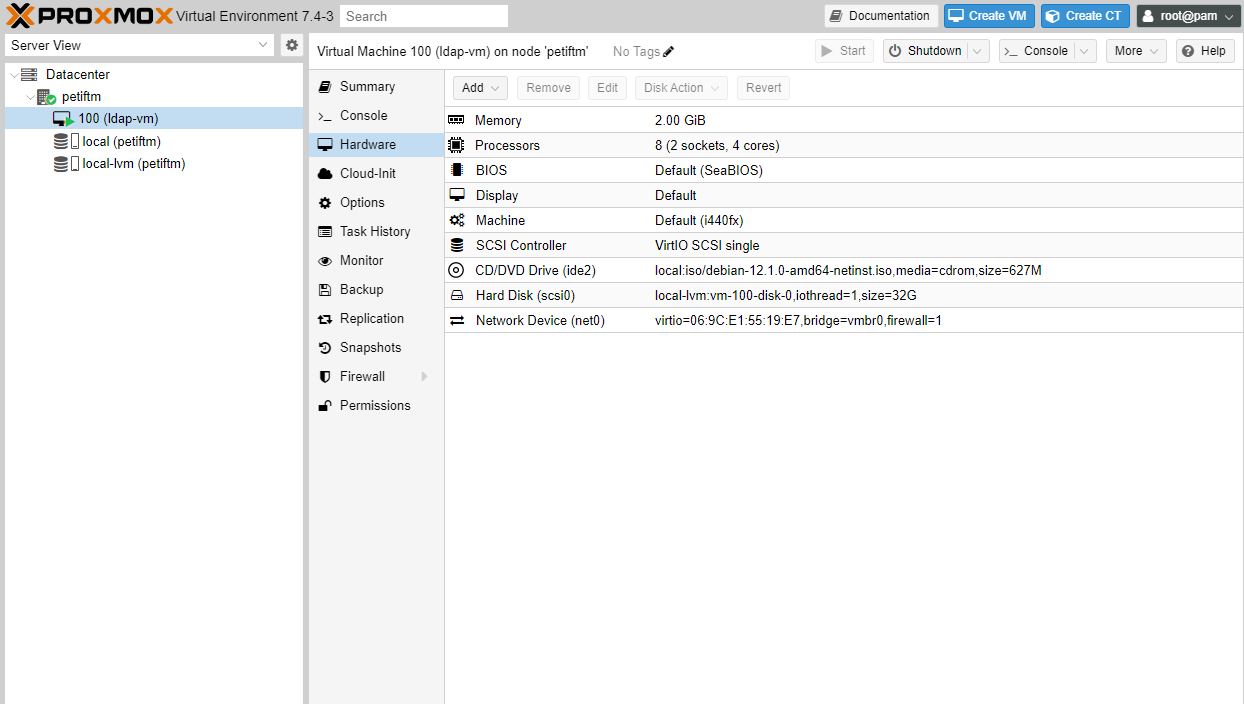
\includegraphics[scale=0.4]{textuais/VMconfigs2.png}
	\caption{Configurações de hardware da máquina virtual Debian}
	\label{fig:hardwareDebian}
\end{figure}

Os requisitos de hardware da VM independem da instalação do OpenLDAP, pois ele é um serviço de diretório leve que pode ser executado em hardware modesto. No entanto, é importante notar que o desempenho do OpenLDAP pode ser afetado pelo hardware subjacente, portanto, quanto melhor for o desempenho esperado, maior deve ser a qualidade do hardware.

